\section{Synthèse des fonctions}

Une fois la validation en simulation des différents blocs effectuée, il est nécessaire de réaliser la synthèse sur FPGA afin d’observer les ressources logiques attribuées à notre système. 
Dans le cadre de ce projet, nous avons utilisé un FPGA \textit{AMD Xilinx Artix-7}, plus précisément le modèle \texttt{7A35TCPG236}. 
L’objectif de cette étape est d’analyser les ressources logiques mobilisées, ainsi que les éléments matériels effectivement utilisés par notre conception.
\newline

\begin{figure}[h]
\centering
\resizebox{\textwidth}{!}{% 
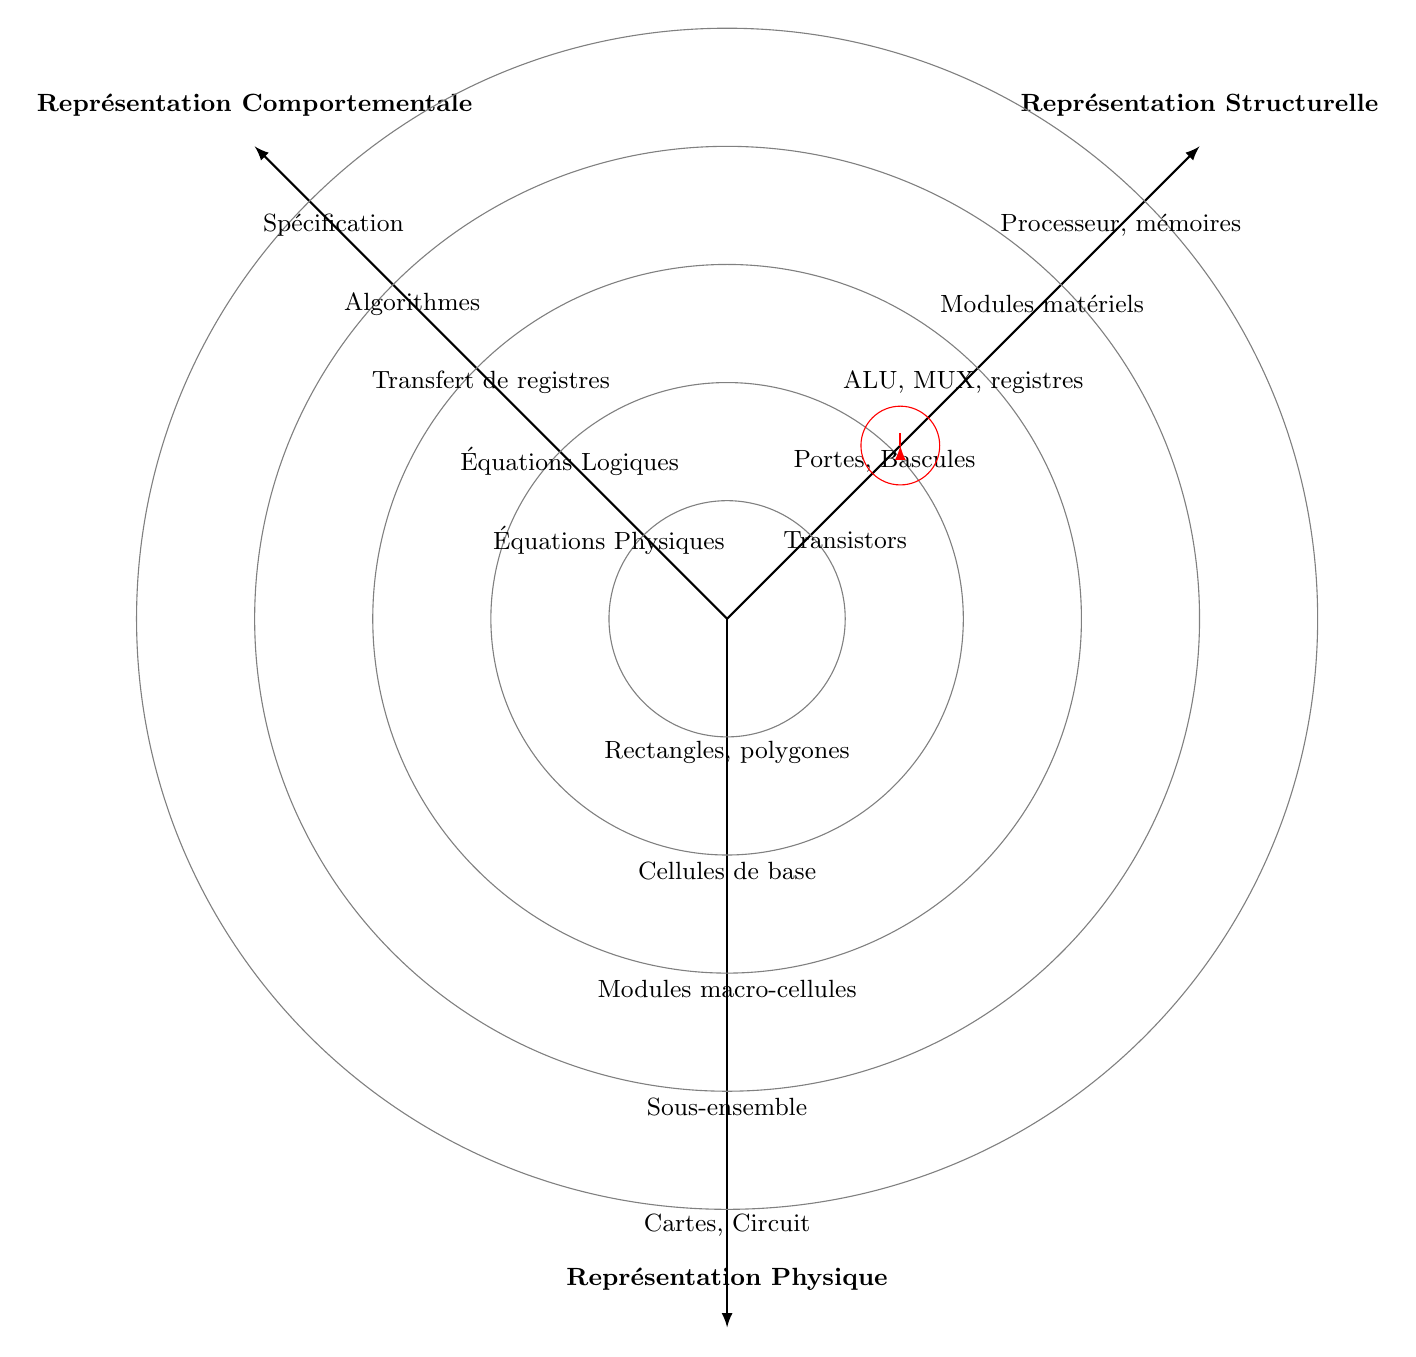
\begin{tikzpicture}[
    axis/.style={thick, -latex},
    font=\small
]

% Définir les coordonnées pour les trois axes
\coordinate (O) at (0,0); % Centre
\coordinate (B) at (-6,6); % Axe Behavioral
\coordinate (S) at (6,6);  % Axe Structural  
\coordinate (P) at (0,-9); % Axe Physical

% Dessiner les axes
\draw[axis] (O) -- (B) node[at end, yshift=15pt] {\textbf{Représentation Comportementale}};
\draw[axis] (O) -- (S) node[at end, yshift=15pt] {\textbf{Représentation Structurelle}};
\draw[axis] (O) -- (P) node[at end, below, yshift=25pt] {\textbf{Représentation Physique}};

% Cercles concentriques
\draw[gray, thin] (O) circle (1.5);
\draw[gray, thin] (O) circle (3);
\draw[gray, thin] (O) circle (4.5);
\draw[gray, thin] (O) circle (6);
\draw[gray, thin] (O) circle (7.5);

% Niveaux sur l'axe Behavioral (côté gauche)
\node[align=center] at (-1.5,1) {Équations Physiques};
\node[align=center] at (-2,2) {Équations Logiques};
\node[align=center] at (-3,3) {Transfert de registres};
\node[align=center] at (-4,4) {Algorithmes};
\node[align=center] at (-5,5) {Spécification};

% Niveaux sur l'axe Structural (côté droit)
\node[align=center] at (1.5,1) {Transistors};
\node[align=center] at (2,2) {Portes, Bascules};
\node[align=center] at (3,3) {ALU, MUX, registres};
\node[align=center] at (4,4) {Modules matériels};    
\node[align=center] at (5,5) {Processeur, mémoires};

% Niveaux sur l'axe Physical (bas)
\node[align=center] at (0,-1.7) {Rectangles, polygones};
\node[align=center] at (0,-3.2) {Cellules de base};
\node[align=center] at (0,-4.7) {Modules macro-cellules};
\node[align=center] at (0,-6.2) {Sous-ensemble};
\node[align=center] at (0,-7.7) {Cartes, Circuit};

% Cercle rouge et flèche de synthèse (boucle sur elle-même)
\draw[red, thin] (2.2,2.2) circle (0.5);
\draw[red, thick, -latex] (2.2,2.2) to[out=60, in=300, looseness=12] (2.2,2.2);

\end{tikzpicture}
}
\caption{Diagramme en Y - Action de synthèse}
\label{fig:diagramme_y_synthese}
\end{figure}

\subsection{Interface Microprocesseur}

Le schéma RTL (\textit{Register Transfer Level}) représente une implémentation 
synthétisée d’un module matériel décrit en VHDL ou Verilog. 
Il illustre les registres, les multiplexeurs, les portes logiques, 
ainsi que la logique séquentielle et combinatoire du circuit.


\begin{figure}[H]
    \centering
    \includegraphics[width=0.9\linewidth]{images/Synthe/RTL_Shematic.png}
    \caption{Schéma RTL InterfaceMicroprocesseur}
    \label{fig:placeholder}
\end{figure}

\subsection*{Structure générale}
Le schéma peut être décomposé en plusieurs parties :
\begin{itemize}
    \item \textbf{Entrées principales} : signaux tels que 
    \texttt{H}, \texttt{CnD}, \texttt{RnW}, \texttt{nRST}, \texttt{nCS}, etc.
    \item \textbf{Registres (Flip-Flops D)} : éléments synchronisés par l’horloge, 
    servant à mémoriser l’état interne du circuit.
    \item \textbf{Multiplexeurs (MUX)} : permettent de sélectionner une donnée 
    parmi plusieurs, selon les conditions de contrôle.
    \item \textbf{Logique combinatoire} : réalisée par des portes AND, OR, NOT 
    et XOR, afin de générer les conditions de transition et les sorties.
    \item \textbf{Sorties} : plusieurs signaux dérivés de l’état interne, 
    comme \texttt{State\_XX}, \texttt{Output\_XX}, etc.
\end{itemize}

\subsection*{Fonctionnement global}
Le circuit implémente une \textbf{machine à états finis} :
\begin{itemize}
    \item Les \textbf{registres} contiennent l’état courant.
    \item La \textbf{logique combinatoire} calcule l’état suivant 
    en fonction de l’état courant et des entrées.
    \item Les \textbf{multiplexeurs} dirigent les transitions entre états.
    \item Les \textbf{sorties} sont activées ou désactivées selon l’état courant 
    et certaines combinaisons d’entrées.
\end{itemize}

\begin{figure}[H]
    \centering
    \includegraphics[width=0.9\linewidth]{images/Synthe/mux_tris.png}
    \caption{Partie opérative avec multiplexeur et Tristate : InterfaceMicroprocesseur}
    \label{fig:placeholder}
\end{figure}

De plus, nous pouvons retrouver la partie opérative dessinée en classe, lors de nos TD, qui permet, 
grâce à un multiplexeur, de sélectionner \textbf{EtalLu} ou \textbf{OctetLu} pour l'envoyer vers 
une porte \textbf{Tristate}.  
Cela démontre la cohérence entre la réalisation théorique et la mise en œuvre pratique.
\newline

À la suite de la synthèse logique nous pouvons avoir la la synthèse matériel qui transforme la 
logique en ressource matérielle.

\begin{figure}[H]
    \centering
    \includegraphics[width=0.9\linewidth]{images/Synthe/RTL_HARD_HDL.jpg}
    \caption{Synthese matérielle InterfaceMicroprocesseur}
    \label{fig:placeholder}
\end{figure}

Cette transformation consiste à mapper les éléments logiques du schéma RTL, tels que les portes 
\textbf{ AND, OR, NOT} ou les \textbf{multiplexeurs}, sur les \textbf{ressources matérielles 
physiques} disponibles dans le FPGA, notamment :  
\newline

\begin{itemize}
    \item \textbf{LUT (Look-Up Tables)} : les fonctions combinatoires, comme les portes logiques ou les multiplexeurs, sont réalisées à l’aide de LUT. Chaque LUT peut implémenter n’importe quelle fonction booléenne sur un nombre limité d’entrées, ce qui permet de reproduire fidèlement la logique définie dans le HDL.
    \item \textbf{Flip-flops} : les éléments séquentiels tels que les registres ou les bascules sont mappés sur des flip-flops pour stocker les bits et synchroniser les signaux dans le temps.
    \item \textbf{Buffers} : certains chemins logiques nécessitent des buffers pour renforcer les signaux ou adapter les niveaux électriques, garantissant ainsi la stabilité et l’intégrité du routage sur la puce.
\end{itemize}

Grâce à cette conversion, le design passe d’une \textbf{représentation abstraite de la logique} à une \textbf{implémentation matérielle concrète}, optimisée pour le FPGA cible. Cela permet non seulement de visualiser l’organisation physique des composants.
\newline

\subsection{Interface Reception Trame}

Comme pour l’Interface Microprocesseur, nous avons le schéma RTL de l’Interface Reception Trame. 
Celui ci représente la machine squénce finie implémentée dans le FPGA. Celui ci nous permet de
visualiser les différents registres, multiplexeurs et portes logiques utilisés pour la conception de cette machine.
\newline

Voici le schéma RTL de l’Interface Reception Trame :

%%%%%%%%%%%%%%%%%%%%%%%%%%%%%%%%%%%%%%%%%%%%%%%%%%%%%%%%%%%%%%%%%%%%%%%%%%%%%%%%%%%%%%%%%%%%%%%%%
%
%\begin{figure}[H]
%    \centering
%    \includegraphics[width=0.9\linewidth]{images/Synthe/RTL_Shematic_IRT.png}
%    \caption{Schéma RTL InterfaceReceptionTrame}
%    \label{fig:RTL_Shematic_IRT}
%\end{figure}
%
%%%%%%%%%%%%%%%%%%%%%%%%%%%%%%%%%%%%%%%%%%%%%%%%%%%%%%%%%%%%%%%%%%%%%%%%%%%%%%%%%%%%%%%%%%%%%%%%%

\subsection*{Structure générale}
Le schéma peut être décomposé en plusieurs parties :
\begin{itemize}
    \item \textbf{Entrées principales} : signaux tels que 
    \texttt{LIN}, \texttt{SeldADR}, \texttt{nCLR}, \texttt{H}, etc.
    \item \textbf{Registres (Flip-Flops D)} : éléments synchronisés par l’horloge, 
    servant à mémoriser l’état interne du circuit.
    \item \textbf{Multiplexeurs (MUX)} : permettent de sélectionner une donnée 
    parmi plusieurs, selon les conditions de contrôle.
    \item \textbf{Logique combinatoire} : réalisée par des portes AND, OR, NOT 
    et XOR, afin de générer les conditions de transition et les sorties.
    \item \textbf{Sorties} : plusieurs signaux de sortie pour la FIFO et l'EtatInterne.
\end{itemize}

\subsection*{Fonctionnement global}

Nous pouvons retrouver la partie opérative dessinée en classe, lors de nos TD, celle ci contenant, des multiplexeurs et des portes logiques,
ainsi que des compteurs/décompteurs.
\newline

Voici la partie opérative de l’Interface Reception Trame :

%%%%%%%%%%%%%%%%%%%%%%%%%%%%%%%%%%%%%%%%%%%%%%%%%%%%%%%%%%%%%%%%%%%%%%%%%%%%%%%%%%%%%%%%%%%%%%%%%
%
%\begin{figure}[H]
%    \centering
%    \includegraphics[width=0.9\linewidth]{images/Synthe/ZOOM_1_RTL_Shematic_RTL.png}
%    \caption{Schéma RTL InterfaceReceptionTrame}
%    \label{fig:ZOOM_1_RTL_Shematic_RTL}
%\end{figure}
%
%%%%%%%%%%%%%%%%%%%%%%%%%%%%%%%%%%%%%%%%%%%%%%%%%%%%%%%%%%%%%%%%%%%%%%%%%%%%%%%%%%%%%%%%%%%%%%%%%

A la suite nous obtenons la synthese matérielle qui nous permet de visualiser les ressources matérielles utilisées pour la conception de cette machine.
\newline

Voici la synthese matérielle de l’Interface Reception Trame :

%%%%%%%%%%%%%%%%%%%%%%%%%%%%%%%%%%%%%%%%%%%%%%%%%%%%%%%%%%%%%%%%%%%%%%%%%%%%%%%%%%%%%%%%%%%%%%%%%
%
%\begin{figure}[H]
%    \centering
%    \includegraphics[width=0.9\linewidth]{images/Synthe/ZOOM_1_RTL_Shematic_RTL.png}
%    \caption{Schéma RTL InterfaceReceptionTrame}
%    \label{fig:ZOOM_1_RTL_Shematic_RTL}
%\end{figure}
%
%%%%%%%%%%%%%%%%%%%%%%%%%%%%%%%%%%%%%%%%%%%%%%%%%%%%%%%%%%%%%%%%%%%%%%%%%%%%%%%%%%%%%%%%%%%%%%%%%

Comme pour l’Interface Microprocesseur, cette transformation consiste à mapper les éléments logiques du schéma RTL, tels que les portes 
\textbf{ AND, OR, NOT} ou les \textbf{multiplexeurs}, sur les \textbf{ressources matérielles 
physiques} disponibles dans le FPGA, notamment :    
\newline

\begin{itemize}
    \item \textbf{LUT (Look-Up Tables)} : les fonctions combinatoires, comme les portes logiques ou les multiplexeurs, sont réalisées à l’aide de LUT. Chaque LUT peut implémenter n’importe quelle fonction booléenne sur un nombre limité d’entrées, ce qui permet de reproduire fidèlement la logique définie dans le HDL.
    \item \textbf{Flip-flops} : les éléments séquentiels tels que les registres ou les bascules sont mappés sur des flip-flops pour stocker les bits et synchroniser les signaux dans le temps.
    \item \textbf{Buffers} : certains chemins logiques nécessitent des buffers pour renforcer les signaux ou adapter les niveaux électriques, garantissant ainsi la stabilité et l’intégrité du routage sur la puce
\end{itemize}

\subsection{FIFO}

Comme pour les deux autres modules, nous avons le schéma RTL de la FIFO : 

%%%%%%%%%%%%%%%%%%%%%%%%%%%%%%%%%%%%%%%%%%%%%%%%%%%%%%%%%%%%%%%%%%%%%%%%%%%%%%%%%%%%%%%%%%%%%%%%%
%
%\begin{figure}[H]
%    \centering
%    \includegraphics[width=0.9\linewidth]{images/Synthe/RTL_Shematic_FIFO.png}
%    \caption{Schéma RTL FIFO}
%    \label{fig:RTL_Shematic_FIFO}
%\end{figure}
%
%%%%%%%%%%%%%%%%%%%%%%%%%%%%%%%%%%%%%%%%%%%%%%%%%%%%%%%%%%%%%%%%%%%%%%%%%%%%%%%%%%%%%%%%%%%%%%%%%

\subsection{EtatInterne}

Comme pour les deux autres modules, nous avons le schéma RTL de la EtatInterne : 

%%%%%%%%%%%%%%%%%%%%%%%%%%%%%%%%%%%%%%%%%%%%%%%%%%%%%%%%%%%%%%%%%%%%%%%%%%%%%%%%%%%%%%%%%%%%%%%%%
%
%\begin{figure}[H]
%    \centering
%    \includegraphics[width=0.9\linewidth]{images/Synthe/RTL_Shematic_ETAT.png}
%    \caption{Schéma RTL EtatInterne}
%    \label{fig:RTL_Shematic_ETAT}
%\end{figure}
%
%%%%%%%%%%%%%%%%%%%%%%%%%%%%%%%%%%%%%%%%%%%%%%%%%%%%%%%%%%%%%%%%%%%%%%%%%%%%%%%%%%%%%%%%%%%%%%%%%

Dans celui ci nous pouvons observer les différents registres, multiplexeurs et portes logiques utilisés pour la conception de cette machine.

%%%%%%%%%%%%%%%%%%%%%%%%%%%%%%%%%%%%%%%%%%%%%%%%%%%%%%%%%%%%%%%%%%%%%%%%%%%%%%%%%%%%%%%%%%%%%%%%%
%
%\begin{figure}[H]
%    \centering
%    \includegraphics[width=0.9\linewidth]{images/Synthe/ZOOM_1_RTL_Shematic_EtatInterne.png}
%    \caption{Schéma RTL EtatInterne}
%    \label{fig:RTL_Shematic_EtatInterne}
%\end{figure}
%
%%%%%%%%%%%%%%%%%%%%%%%%%%%%%%%%%%%%%%%%%%%%%%%%%%%%%%%%%%%%%%%%%%%%%%%%%%%%%%%%%%%%%%%%%%%%%%%%%

Nous observons une bascule D qui permet de socket l'erreur de bit Synchro, comme vu dans la partie TD.

\subsection{Reception LIN}

A la suite nous avons décider d'observer le schéma RTL de la Reception LIN, celui ci regroupans tous les systemes précédents.
Dans ce schéma nous allons retrouver les différents blocs que nous avons synthétisé précédemment, à savoir :
\begin{itemize}
    \item Interface Microprocesseur
    \item Interface Reception Trame
    \item FIFO
    \item EtatInterne
\end{itemize}

%%%%%%%%%%%%%%%%%%%%%%%%%%%%%%%%%%%%%%%%%%%%%%%%%%%%%%%%%%%%%%%%%%%%%%%%%%%%%%%%%%%%%%%%%%%%%%%%%
%
%\begin{figure}[H]
%    \centering
%    \includegraphics[width=0.9\linewidth]{images/Synthe_RTL_Shematic_Reception.png}
%    \caption{Schéma RTL Reception LIN}
%    \label{fig:RTL_Shematic_Reception}
%\end{figure}
%%%%%%%%%%%%%%%%%%%%%%%%%%%%%%%%%%%%%%%%%%%%%%%%%%%%%%%%%%%%%%%%%%%%%%%%%%%%%%%%%%%%%%%%%%%%%%%%%%

Ce schéma nous permet d'observer toute les ressources logiques utilisées pour la conception de notre projet. 
\newline
